
\chapter{Ugeopgave 8}
\label{cha:ugeopgave-8}

\section{Part 1}

N�r vi compiler programmet fra start f�r vi en animation, hvorfra et
screenshot kan ses p� figur \ref{fig:8-1-1}.

\begin{figure}[hp]
\centering
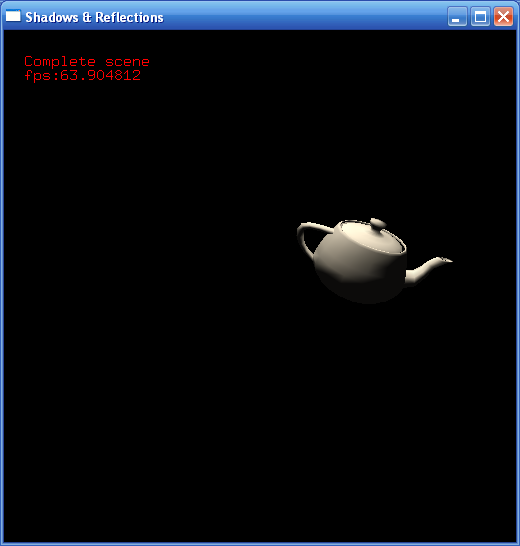
\includegraphics[width=8cm]{../exercise8/screenshots/1.png}
\caption{Det udleverede program}
\label{fig:8-1-1}
\end{figure}


\section{Part 2}

Vi skal nu implementere 2 funktioner:

\texttt{set\_from\_light\_perspective(...)}\\
Funktionen laver en ``perspective projection'' som passer til objektet
ud fra dens ``bounding sphere''.


\texttt{init\_proj\_shadow\_texture(...)}\\
Initialiserer en texture som indeholder skyggen, opretter et texture
name og ops�tter filters.

\section{Part 3}

\paragraph{\texttt{make\_proj\_shadow\_texture(...)}}

Tepotten renderes fra lyskilden og kopierer framebufferen til en
textur.

\begin{figure}[hp]
\centering
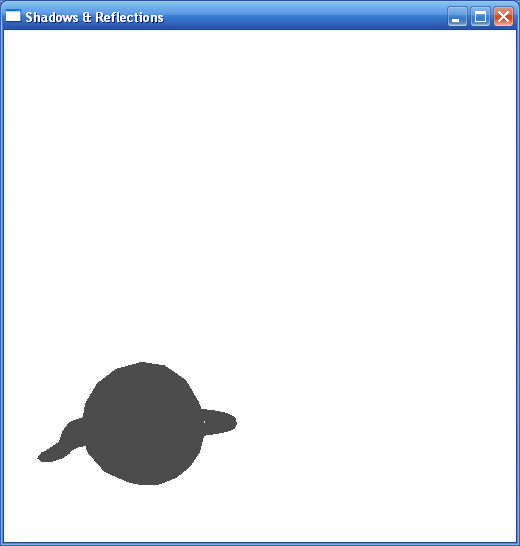
\includegraphics[width=8cm]{../exercise8/screenshots/3.png}
\caption{Skyggen}
\label{fig:8-3-1}
\end{figure}

\section{Part 4}

\paragraph{\texttt{draw\_proj\_shadow(...)}}

Til sidst s�ttes det hele sammen. Farven i frame bufferen blandes med texturen.

Der er tilf�jet et clipping plane, s� skyggen ikke bliver vist hvis
tepotten er under gulvet. Dette skal bruges i exercise 10.

Et screenshot af dette kan ses p� figur \ref{fig:4-3-1}.

\begin{figure}[hp]
\centering
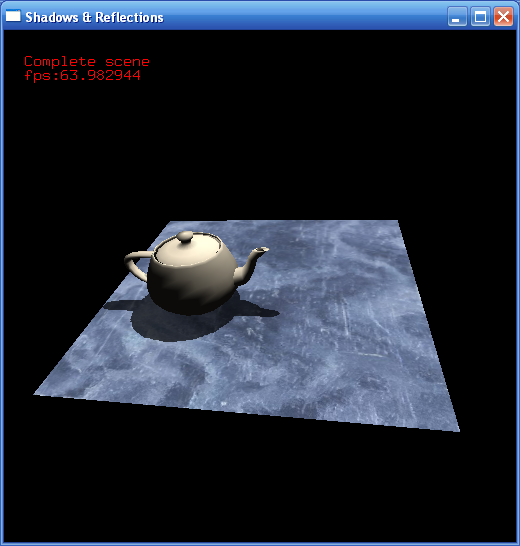
\includegraphics[width=8cm]{../exercise8/screenshots/4.png}
\caption{Det f�rdige program}
\label{fig:4-3-1}
\end{figure}

%%% Local Variables: 
%%% mode: latex
%%% TeX-master: "report_main"
%%% End: 